\documentclass[answers]{exam} % Clase para exámenes con respuestas
\usepackage[english,spanish]{babel} % Soporte para inglés y español
\usepackage[autostyle]{csquotes} % Manejo de citas
\usepackage{amsmath, amssymb} % Paquetes para matemáticas avanzadas
\usepackage{graphicx} % Inclusión de gráficos
\usepackage{enumitem} % Personalización de listas enumeradas
\usepackage[letterpaper,top=2cm,bottom=2cm,left=1.5cm,right=1.5cm]{geometry} % Márgenes ajustados para mayor ancho de contenido
\usepackage[colorlinks=true, allcolors=blue]{hyperref} % Enlaces con color

\usepackage{array}   % for adjusting row height
\renewcommand{\arraystretch}{1.5} % adjust the vertical spacing between rows
\usepackage{multicol}
\usepackage{babel}
\usepackage{tikz}
\usetikzlibrary{babel}

\renewcommand{\solutiontitle}{\noindent\textbf{Respuesta:}\par\noindent} % Personalización del título de respuestas
\renewcommand{\familydefault}{\sfdefault}

% Configuración de encabezado y pie de página
\pagestyle{headandfoot}
\firstpageheader{Universidad de Bolívar}{}{17 de Septiembre del 2024} 
\runningheader{Universidad de Bolívar}{}{Física}
\firstpagefooter{}{\thepage}{}
\runningfooter{}{\thepage}{}

\begin{document}

\begin{center}
	\large\textbf{Trabajo Autónomo 1.2 - Fundamentos de Física para Ingeniería}\\[1em]
	\large Segundo Ciclo \enquote*{A} - Ingeniería de Software\\[1em]
\end{center}

\vspace{0.5cm}
\large\textbf{Estudiante:} Ariel Alejandro Calderón
\vspace{0.5cm}

\begin{questions}

	% Question 1
	\question \large\textbf{Encontrar la fórmula que determina la carga total de un cubo de lado $\alpha$, cuya carga se encuentra distribuida uniformemente solo en las caras superficiales con densidad superficial $\sigma$. Determinar el valor para el caso $\alpha = 0.2 m$ $\sigma = 106C/m^2$.}

	\vspace{0.5cm}



	\begin{multicols}{2} % Inicia el entorno de dos columnas
		La carga total \( Q \) distribuida uniformemente
		\[
			Q = \sigma \cdot A_{\text{total}}
		\]
		donde \( A_{\text{total}} \) es el área total de las superficies del cubo. Para un cubo de lado \( \alpha \), el área total es:
		\[
			A_{\text{total}} = 6 \alpha^2
		\]

		Entonces, la carga total es:
		\[
			Q = \sigma \cdot 6 \alpha^2
		\]

		Sustituyendo los valores dados, con \( \alpha = 0.2 \, \text{m} \) y \( \sigma = 10^6 \, \text{C/m}^2 \):
		\[
			Q = 10^6 \, \text{C/m}^2 \cdot 6 \cdot (0.2 \, \text{m})^2
		\]

		Calculamos \( (0.2)^2 = 0.04 \):
		\[
			Q = 10^6 \cdot 6 \cdot 0.04 = 10^6 \cdot 0.24 = 2.4 \times 10^5 \, \text{C}
		\]

		Por lo tanto, la carga total \( Q \) es:
		\[
			Q = 2.4 \times 10^5 \, \text{C}
		\]
	\end{multicols}

	\begin{minipage}{\textwidth}
		\centering
		\begin{tikzpicture}
			\pgfmathsetmacro{\cubex}{2}
			\pgfmathsetmacro{\cubey}{2}
			\pgfmathsetmacro{\cubez}{2}
			\draw[black,fill=yellow] (0,0,0) -- ++(-\cubex,0,0) -- ++(0,-\cubey,0) -- ++(\cubex,0,0) -- cycle;
			\draw[black,fill=yellow] (0,0,0) -- ++(0,0,-\cubez) -- ++(0,-\cubey,0) -- ++(0,0,\cubez) -- cycle;
			\draw[black,fill=yellow] (0,0,0) -- ++(-\cubex,0,0) -- ++(0,0,-\cubez) -- ++(\cubex,0,0) -- cycle;
		\end{tikzpicture}
		$\alpha$
	\end{minipage}

	\vspace{0.5cm}

	% Question 2
	\question \large\textbf{Encuentre la carga total de un alambre delgado de 2 m de longitud paralelo al eje x que se encuentra cargado con densidad lineal de carga $\lambda = (e^x + x) C/m$  }

	\vspace{0.5cm}

	\begin{multicols}{2} % Inicia el entorno de dos columnas
		La densidad lineal de carga es:
		\[
			\lambda(x) = e^x + x \, \text{C/m}
		\]
		y el alambre tiene una longitud de \( L = 2 \, \text{m} \).

		La carga total \( Q \) se obtiene integrando la densidad lineal de carga a lo largo de la longitud del alambre:
		\[
			Q = \int_0^2 \lambda(x) \, dx = \int_0^2 (e^x + x) \, dx
		\]

		Calculamos la integral:
		\[
			Q = \int_0^2 e^x \, dx + \int_0^2 x \, dx
		\]

		Primera integral:
		\[
			\int_0^2 e^x \, dx = e^2 - e^0 = e^2 - 1
		\]
		Segunda integral:
		\[
			\int_0^2 x \, dx = \frac{x^2}{2} \Bigg|_0^2 = \frac{2^2}{2} = 2
		\]

		Entonces, la carga total es:
		\[
			Q = (e^2 - 1) + 2
		\]

		Obtenemos:
		\[
			Q = (7.389 - 1) + 2 = 6.389 + 2 = 8.389 \, \text{C}
		\]
	\end{multicols}

	\vspace{0.5cm}

	% Question 3
	\question \large\textbf{Dos esferas de masa 1gr y de igual carga Q se cuelgan de hilos de 20cm y masa despreciable sujetos a un mismo punto. Si el ángulo que forman los hilos en el punto
		común es de $20^{\circ}$, calcular el valor de Q.  }

	\begin{multicols}{2} % Inicia el entorno de dos columnas

		La fuerza de repulsión electrostática entre las esferas \( F_e \) es responsable de mantener el ángulo \( 20^\circ \). Por otro lado, el peso de cada esfera \( W \) actúa hacia abajo, y la tensión en los hilos tiene una componente vertical que equilibra el peso y una componente horizontal que equilibra la fuerza electrostática.

		La fórmula de la fuerza electrostática entre dos cargas es:
		\[
			F_e = k_e \frac{Q^2}{r^2}
		\]
		donde \( k_e \) es la constante de Coulomb (\( 9 \times 10^9 \, \text{Nm}^2/\text{C}^2 \)) y \( r \) es la distancia entre las esferas. La distancia \( r \) entre las esferas se puede calcular en función del ángulo \( \theta = 20^\circ \) y la longitud del hilo \( L = 20 \, \text{cm} \):
		\[
			\sin\left(\frac{\theta}{2}\right) = \dfrac{\frac{r}{2}}{L}\implies r = 2L \sin\left(\frac{\theta}{2}\right)
		\]

		Sustituyendo \( L = 0.2 \, \text{m} \) y \( \theta = 20^\circ \):
		\[
			r = 2(0.2) \sin\left(10^\circ\right) \approx 0.0698 \, \text{m}
		\]

		Ahora, igualamos la componente horizontal de la tensión \( T \) con la fuerza electrostática:
		\[
			\sum F_x = 0  \implies T \sin\left(10^\circ\right) = F_e
		\]

		También, la componente vertical de la tensión equilibra el peso \( W = mg \), donde \( m = 1 \, \text{g} = 0.001 \, \text{kg} \) y \( g = 9.8 \, \text{m/s}^2 \):
		\[
			\sum F_y = 0  \implies T \cos\left(10^\circ\right) = W
		\]
		\[
			T  = \dfrac{mg}{\cos\left(10^\circ\right)} \implies F_e = mg\cdot \tan\left(10^\circ\right)
		\]

		Resolviendo ambas ecuaciones para \( Q \), obtenemos:
		\[
			Q = \sqrt{\frac{r^2 \cdot F_e}{k_e}} = \sqrt{\frac{(0.0698)^2 (0.001)(9.8) \tan(10^\circ)}{9 \times 10^9}}
		\]

		Aproximando los valores:
		\[
			Q \approx 1.21 \times 10^{-8} \, \text{C}
		\]
	\end{multicols}

	\begin{multicols}{2}
		\begin{minipage}{\textwidth}
			\begin{tikzpicture}[scale=1]
				% Dibujar las cuerdas
				\draw[thick] (0,0) -- (-1,-2) node[midway, right] {$20^\circ$};
				\draw[thick] (0,0) -- (1,-2);
	
				% Dibujar las esferas
				\shade[ball color=blue] (-1,-2) circle (0.1);
				\shade[ball color=blue] (1,-2) circle (0.1);
	
				% Dibujar etiquetas de las cargas
				\node at (-1.3,-2.3) {$Q$};
				\node at (1.3,-2.3) {$Q$};
	
			\end{tikzpicture}
			% \caption{Esferas suspendidas con cargas \( Q \)}
		\end{minipage}

<<<<<<< HEAD
		\begin{minipage}{\textwidth}
			
			\begin{tikzpicture}[scale=1]
				% Dibujar las esferas
				\shade[ball color=blue] (-1,-2) circle (0.9);
				% Componentes
				\draw[dashed,->] (-1,-2) -- (1.5,0);
				% Ejes
				\draw[->] (-1,-2) -- (-1,0);
				\draw[->] (-1,-2) -- (-1,-4);
				\draw[->] (-1,-2) -- (2,-2);

				\node at (-1.3,-2.3) {$Q$};
				\node at (1.3,-2.3) {$Q$};


			\end{tikzpicture}
			% \caption{Esferas suspendidas con cargas \( Q \)}
		\end{minipage}
	\end{multicols}
=======
	\begin{minipage}{\textwidth}
		\centering
		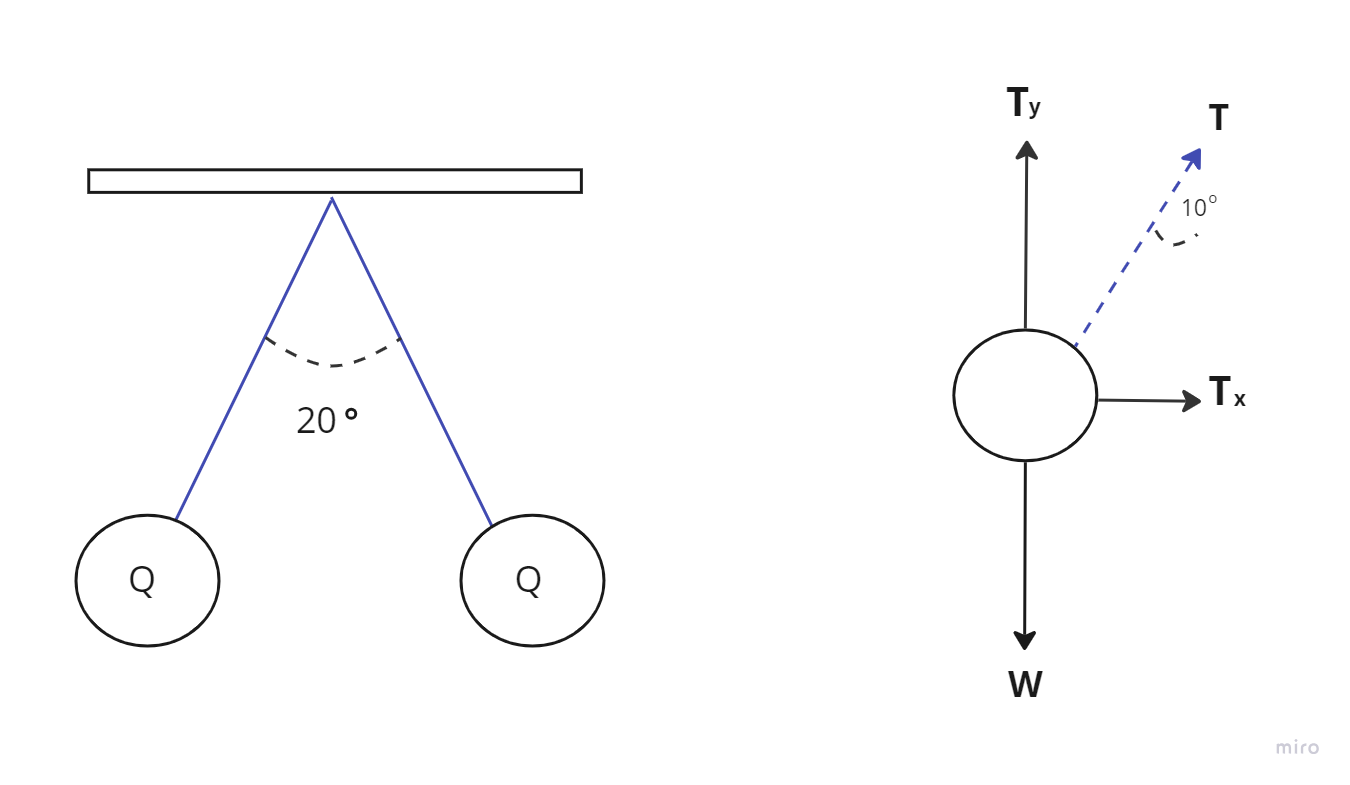
\includegraphics[width=0.9\textwidth]{public/g3.png}\\
	\end{minipage}
>>>>>>> faa70998f42655185a0185d34fbb2808f7bb0545

	\vspace{0.5cm}
	\newpage

	\newpage

	% Question 4
	\question \large\textbf{Tres cargas puntuales se ubican a lo largo del eje x. Q1= 1mC está en x = 1m ,  Q2 = 2 x $10^{-6}$C en x = 2m. Dónde debe ubicarse la tercera carga Q3 positiva de modo que
		ésta última carga se mantenga estática.}

	\begin{multicols}{2} % Inicia el entorno de dos columnas

		Para que la tercera carga \( Q_3 \) esté en equilibrio, la fuerza que ejerce \( Q_1 \) sobre \( Q_3 \) debe ser igual a la fuerza que ejerce \( Q_2 \) sobre \( Q_3 \). Aplicamos la ley de Coulomb para ambas fuerzas:

		\[
			F = k_e \frac{|Q_i Q_j|}{r^2}
		\]

		Por lo tanto, el equilibrio de fuerzas se expresa como:

		\[
			|\vec{F_{13}}| = |\vec{F_{23}}|
		\]

		\[
			k_e \dfrac{|Q_1 Q_3|}{|\vec{r_{13}}|^2} = k_e \dfrac{|Q_2 Q_3|}{|\vec{r_{23}}|^2}
		\]

		\[
			k_e \dfrac{|Q_1 Q_3|}{(x_3 - x_1)^2} = k_e \dfrac{|Q_2 Q_3|}{(x_3 - x_2)^2}
		\]

		\[
			\frac{|Q_1|}{(x_3 - x_1)^2} = \frac{|Q_2|}{(x_3 - x_2)^2}
		\]

		\[
			\frac{1 \times 10^{-3}}{(x_3 - 1)^2} = \frac{2 \times 10^{-6}}{(x_3 - 2)^2}
		\]

		\[
			1 \times 10^{-3} (x_3 - 2)^2 = 2 \times 10^{-6} (x_3 - 1)^2
		\]


		\[
			500 (x_3 - 2)^2 = (x_3 - 1)^2
		\]

		\[
			\sqrt{500} (x_3 - 2) = x_3 - 1
		\]

		\[
			21.36 x_3 = 43.72
		\]

		\[
			x_3 = \frac{43.72}{21.36} \approx 2.05 \, \text{m}
		\]
	\end{multicols}

<<<<<<< HEAD

	\begin{minipage}{\textwidth}
		\centering
		\begin{tikzpicture}[scale=1]
			% Dibujar el eje x
			% \draw[thick,->] (-1,0) -- (5,0) node[right] {$x$};
			\draw[thick] (-1,0) -- (5,0) node[right] {$x$};

			% Posiciones de las cargas Q1, Q2 y Q3
			% \node at (1,0) [below] {$Q_1 = 1 \, \text{mC}$};
			% \node at (2,0) [below] {$Q_2 = 2 \times 10^{-6} \, \text{C}$};
			% \node at (3.5,0) [below] {$Q_3$};

			% Dibujar las fuerzas
			% \draw[->, thick] (3.5,0) -- (1,0) node[midway, above] {$F_{13}$};
			% \draw[->, thick] (2,0) -- (3.5,0) node[midway, above] {$F_{23}$};
			% \draw[ thick] (3.5,0) -- (1,0) node[midway, above] {$F_{13}$};
			% \draw[ thick] (2,0) -- (3.5,0) node[midway, above] {$F_{23}$};

			% Dibujar las cargas
			\shade[ball color=blue] (1,0) circle (0.1);
			\shade[ball color=red] (2,0) circle (0.1);
			\shade[ball color=green] (3.5,0) circle (0.1);
		\end{tikzpicture}
		% \caption{Posición de las cargas en el eje \( x \)}
	\end{minipage}

=======
>>>>>>> faa70998f42655185a0185d34fbb2808f7bb0545
	\vspace{0.5cm}

	\begin{minipage}{\textwidth}
		\centering
		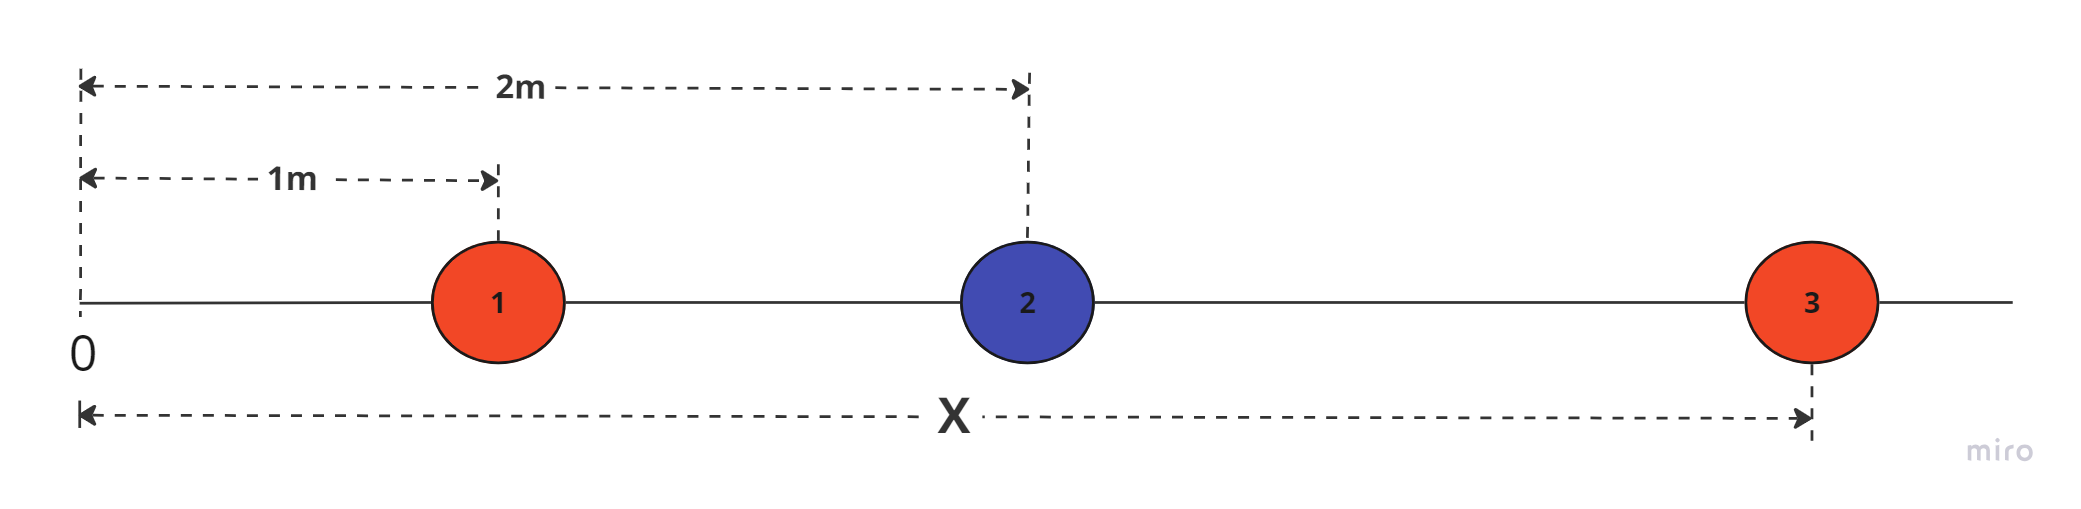
\includegraphics[width=0.9\textwidth]{public/g4.png}\\
	\end{minipage}

	\vspace{0.5cm}
	\newpage
	% % Question 5
	\question \large\textbf{Calcular la fuerza electrostática que produce un anillo de radio a, cargado con densidad lineal $\lambda$, sobre una carga ubicada a una distancia b del centro del anillo sobre su eje. }
	\begin{multicols}{2}
		La configuración es un triángulo equilátero, por lo que las tres distancias entre las cargas son iguales: \( r = 0.5 \, \text{m} \).

		Para encontrar la fuerza neta sobre \( Q_1 \), debemos calcular las fuerzas ejercidas sobre \( Q_1 \) por \( Q_2 \) y \( Q_3 \), y luego sumarlas vectorialmente.

		La fuerza electrostática entre dos cargas está dada por la ley de Coulomb:
		\[
			F = k_e \frac{|Q_i Q_j|}{r^2}
		\]
		donde \( k_e = 9 \times 10^9 \, \text{Nm}^2/\text{C}^2 \).

		\textbf{Fuerza de \( Q_2 \) sobre \( Q_1 \)}
		\[
			F_{21} = k_e \frac{|2 \times 10^{-6} \times (-3 \times 10^{-6})|}{(0.5)^2}
		\]
		\[
			F_{21} = 9 \times 10^9 \frac{6 \times 10^{-12}}{0.25} = 0.216 \, \text{N}
		\]
		La dirección de esta fuerza es hacia \( Q_2 \).

		\textbf{Fuerza de \( Q_3 \) sobre \( Q_1 \):}
		\[
			F_{31} = k_e \frac{|2 \times 10^{-6} \times 1 \times 10^{-6}|}{(0.5)^2}
		\]
		\[
			F_{31} = 9 \times 10^9 \frac{2 \times 10^{-12}}{0.25} = 0.072 \, \text{N}
		\]
		La dirección de esta fuerza es hacia \( Q_3 \).

		\textbf{Suma vectorial de fuerzas}: Dado que el triángulo es equilátero, las fuerzas están separadas por ángulos de \( 60^\circ \). Utilizamos descomposición en componentes para obtener la fuerza neta.

		La fuerza neta sobre \( Q_1 \) es:
		\[
			F_{\text{net}} = F_{21} + F_{31}
		\]
	\end{multicols}

	\begin{minipage}{\textwidth}
		\centering
		\begin{tikzpicture}[scale=1]
			% Dibujar el triángulo equilátero
			\draw[thick] (0,0) -- (2,0) -- (1,1.732) -- cycle;

			% Dibujar las cargas
			\shade[ball color=red] (0,0) circle (0.1) node[below left] {$Q_1 = 2 \, \mu C$};
			\shade[ball color=blue] (2,0) circle (0.1) node[below right] {$Q_2 = -3 \, \mu C$};
			\shade[ball color=green] (1,1.732) circle (0.1) node[above] {$Q_3 = 1 \, \mu C$};

			% Dibujar fuerzas
			\draw[thick] (0,0) -- (2,0) node[midway, below] {$F_{21}$};
			\draw[thick] (0,0) -- (1,1.732) node[midway, right] {$F_{31}$};
		\end{tikzpicture}
		% \caption{Distribución de cargas en un triángulo equilátero}
	\end{minipage}



	\vspace{0.5cm}

\end{questions}

\end{document}